\documentclass[10pt]{article}\usepackage{graphicx, color}
%% maxwidth is the original width if it is less than linewidth
%% otherwise use linewidth (to make sure the graphics do not exceed the margin)
\makeatletter
\def\maxwidth{ %
  \ifdim\Gin@nat@width>\linewidth
    \linewidth
  \else
    \Gin@nat@width
  \fi
}
\makeatother

\definecolor{fgcolor}{rgb}{0.2, 0.2, 0.2}
\newcommand{\hlnumber}[1]{\textcolor[rgb]{0,0,0}{#1}}%
\newcommand{\hlfunctioncall}[1]{\textcolor[rgb]{0.501960784313725,0,0.329411764705882}{\textbf{#1}}}%
\newcommand{\hlstring}[1]{\textcolor[rgb]{0.6,0.6,1}{#1}}%
\newcommand{\hlkeyword}[1]{\textcolor[rgb]{0,0,0}{\textbf{#1}}}%
\newcommand{\hlargument}[1]{\textcolor[rgb]{0.690196078431373,0.250980392156863,0.0196078431372549}{#1}}%
\newcommand{\hlcomment}[1]{\textcolor[rgb]{0.180392156862745,0.6,0.341176470588235}{#1}}%
\newcommand{\hlroxygencomment}[1]{\textcolor[rgb]{0.43921568627451,0.47843137254902,0.701960784313725}{#1}}%
\newcommand{\hlformalargs}[1]{\textcolor[rgb]{0.690196078431373,0.250980392156863,0.0196078431372549}{#1}}%
\newcommand{\hleqformalargs}[1]{\textcolor[rgb]{0.690196078431373,0.250980392156863,0.0196078431372549}{#1}}%
\newcommand{\hlassignement}[1]{\textcolor[rgb]{0,0,0}{\textbf{#1}}}%
\newcommand{\hlpackage}[1]{\textcolor[rgb]{0.588235294117647,0.709803921568627,0.145098039215686}{#1}}%
\newcommand{\hlslot}[1]{\textit{#1}}%
\newcommand{\hlsymbol}[1]{\textcolor[rgb]{0,0,0}{#1}}%
\newcommand{\hlprompt}[1]{\textcolor[rgb]{0.2,0.2,0.2}{#1}}%

\usepackage{framed}
\makeatletter
\newenvironment{kframe}{%
 \def\at@end@of@kframe{}%
 \ifinner\ifhmode%
  \def\at@end@of@kframe{\end{minipage}}%
  \begin{minipage}{\columnwidth}%
 \fi\fi%
 \def\FrameCommand##1{\hskip\@totalleftmargin \hskip-\fboxsep
 \colorbox{shadecolor}{##1}\hskip-\fboxsep
     % There is no \\@totalrightmargin, so:
     \hskip-\linewidth \hskip-\@totalleftmargin \hskip\columnwidth}%
 \MakeFramed {\advance\hsize-\width
   \@totalleftmargin\z@ \linewidth\hsize
   \@setminipage}}%
 {\par\unskip\endMakeFramed%
 \at@end@of@kframe}
\makeatother

\definecolor{shadecolor}{rgb}{.97, .97, .97}
\definecolor{messagecolor}{rgb}{0, 0, 0}
\definecolor{warningcolor}{rgb}{1, 0, 1}
\definecolor{errorcolor}{rgb}{1, 0, 0}
\newenvironment{knitrout}{}{} % an empty environment to be redefined in TeX

\usepackage{alltt}
\usepackage{xcolor}
\usepackage{amsmath}
\usepackage{amstext}
\usepackage{graphicx}
\usepackage{color}        
\usepackage{multirow}
\usepackage{setspace}
\setlength{\parindent}{0in}
\setlength{\parskip}{\baselineskip}

\usepackage[left=1in,top=1.25in,right=1in,bottom=1.25in]{geometry}

\newcommand{\bq}{\begin{quote}\color{blue}}
\newcommand{\eq}{\end{quote}}

\newcommand{\bc}{\begin{center}}
\newcommand{\ec}{\end{center}}

\newcommand{\bra}{\left\langle}
\newcommand{\ket}{\right\rangle}

\newcommand{\ben}{\begin{enumerate}}
\newcommand{\een}{\end{enumerate}}
\newcommand{\I}{\item}

\newcommand{\beq}{\begin{eqnarray}}
\newcommand{\eeq}{\end{eqnarray}}
\newcommand{\ed}{\end{document}}

\newcommand{\PlotH}[2]{\includegraphics[height=#1\textheight]{#2}}
\newcommand{\PlotW}[2]{\includegraphics[width=#1\textwidth]{#2}}
\newcommand{\MultiPlotH}[3]{\includegraphics[height=#1\textheight, page=#2]{#3}}
\newcommand{\MultiPlotW}[3]{\includegraphics[width=#1\textwidth, page=#2]{#3}}

\title{Comparison of methods for identifying behavioral changes in movement data}
\author{Eli Gurarie\\
Co-authors: (provisional) Maria Delgado, Chloe Bracis, \\ 
Ilpo Kojola, Jyrki Pusenius, Michael Wagner, Trevor Meckley, \\
Cl\'ement Calenge, Bram van Moorter, Manuela Panzacchi}
\IfFileExists{upquote.sty}{\usepackage{upquote}}{}


\begin{document}





\maketitle

\emph{ This report is a preliminary analysis for  paper: ``What is the animal doing?  Reviewing techniques for behavioral analysis of remotely sensed animal movements.'' for a special issue in \emph{Animal Ecology}, provisionally with the coauthors listed above.}

\section{Background}

I compared the results of three different kinds of behavioral chagne analyses on three datasets.  In order to make these comparisons more efficient, I bundled the raw data and some specialized wrapper functions into an R package called `waddle`.  In this document, I walk (sketchily) through the analysis methods and the comparison - including the code and output (so that anyone can theoretically replicate the analysis).  This should be the meat of the Methods/Results portion of the paper.  



\section{Materials and Methods}

\subsection{Data}

The data below are presented, very roughly, from "simplest" to most "complex".  All the data are bundled in this package: 
\begin{knitrout}
\definecolor{shadecolor}{rgb}{0.969, 0.969, 0.969}\color{fgcolor}\begin{kframe}
\begin{alltt}
\hlfunctioncall{require}(waddle)
\end{alltt}
\end{kframe}
\end{knitrout}

which itself depends on \texttt{adehabitatLT} and on (my own) \texttt{bcpa} package.


\subsubsection{Lamprey}  

One acoustically tagged sea lamprey \emph{Petromyzon marinus} from Hammond Bay, Lake Huron in 2010 (data from M. Wagner and Michigan State University).  These data include one 12 hour bout with locations collected approximately once per minute.  The lamprey data is behaviorally the simplest: it swims for a while, settles for several hours, and starts swimming again. There may be some additional questions related to whether its swimming behavior can be classified into distinct modes.  

\begin{knitrout}
\definecolor{shadecolor}{rgb}{0.969, 0.969, 0.969}\color{fgcolor}\begin{kframe}
\begin{alltt}
\hlfunctioncall{data}(Lamprey)
\hlfunctioncall{str}(Lamprey)
\end{alltt}
\begin{verbatim}
## Classes 'track' and 'data.frame':	433 obs. of  5 variables:
##  $ Time : POSIXct, format: "2010-05-02 08:49:00" "2010-05-02 08:51:00" ...
##  $ X    : num  728207 728240 728264 728294 728326 ...
##  $ Y    : num  5042248 5042193 5042167 5042147 5042139 ...
##  $ Z    : cplx  728207+5042248i 728240+5042193i 728264+5042167i ...
##  $ Depth: num  1.98 4.62 4.62 4.4 4.62 ...
\end{verbatim}
\begin{alltt}
\hlfunctioncall{diff}(\hlfunctioncall{range}(Lamprey$Time))
\end{alltt}
\begin{verbatim}
## Time difference of 11.33 hours
\end{verbatim}
\end{kframe}
\end{knitrout}


\subsubsection{Wolf} 

One GPS collared wolf (\emph{Canis lupus}, id: Herkules) from Finland, that exhibited a wide-ranging dispersal over an 11 month period, essentially encircling an area of about 160,000 km$^2$  (data: I. Kojola, RKTL). The wolf alternates between periods of rapid dispersal and semi-territorial behaviors. 
\begin{knitrout}
\definecolor{shadecolor}{rgb}{0.969, 0.969, 0.969}\color{fgcolor}\begin{kframe}
\begin{alltt}
\hlfunctioncall{data}(Wolf)
\hlfunctioncall{str}(Wolf)
\end{alltt}
\begin{verbatim}
## Classes 'track' and 'data.frame':	1401 obs. of  3 variables:
##  $ Time: POSIXlt, format: "2005-03-23" "2005-03-24" ...
##  $ X   : num  572 569 568 568 569 ...
##  $ Y   : num  7071 7072 7072 7071 7070 ...
\end{verbatim}
\begin{alltt}
\hlfunctioncall{diff}(\hlfunctioncall{range}(Wolf$Time))
\end{alltt}
\begin{verbatim}
## Time difference of 316 days
\end{verbatim}
\end{kframe}
\end{knitrout}


\subsubsection{Wild forest reindeer} 

One GPS collared wild forest reindeer (\emph{Rangifer tarandus fennicus}) from eastern Finland over a 2.6 year period (data: J. Pusenius, RKTL). The reindeer appears to have multiple ``centers of attraction'', and an overall relatively constrained area (maximum E-W displacement 75 km, maximum N-S displacement 102 km).
\begin{knitrout}
\definecolor{shadecolor}{rgb}{0.969, 0.969, 0.969}\color{fgcolor}\begin{kframe}
\begin{alltt}
\hlfunctioncall{data}(WFR)
\hlfunctioncall{str}(WFR)
\end{alltt}
\begin{verbatim}
## Classes 'track' and 'data.frame':	4974 obs. of  3 variables:
##  $ Time: POSIXct, format: "2009-02-03 23:00:50" "2009-02-04 03:00:43" ...
##  $ X   : num  3578 3578 3578 3578 3578 ...
##  $ Y   : num  7108 7108 7108 7108 7108 ...
\end{verbatim}
\begin{alltt}
\hlfunctioncall{diff}(\hlfunctioncall{range}(WFR$Time))
\end{alltt}
\begin{verbatim}
## Time difference of 946.6 days
\end{verbatim}
\end{kframe}
\end{knitrout}


These data objects are all given a "track" class, which can be easily plotted:

\begin{knitrout}
\definecolor{shadecolor}{rgb}{0.969, 0.969, 0.969}\color{fgcolor}
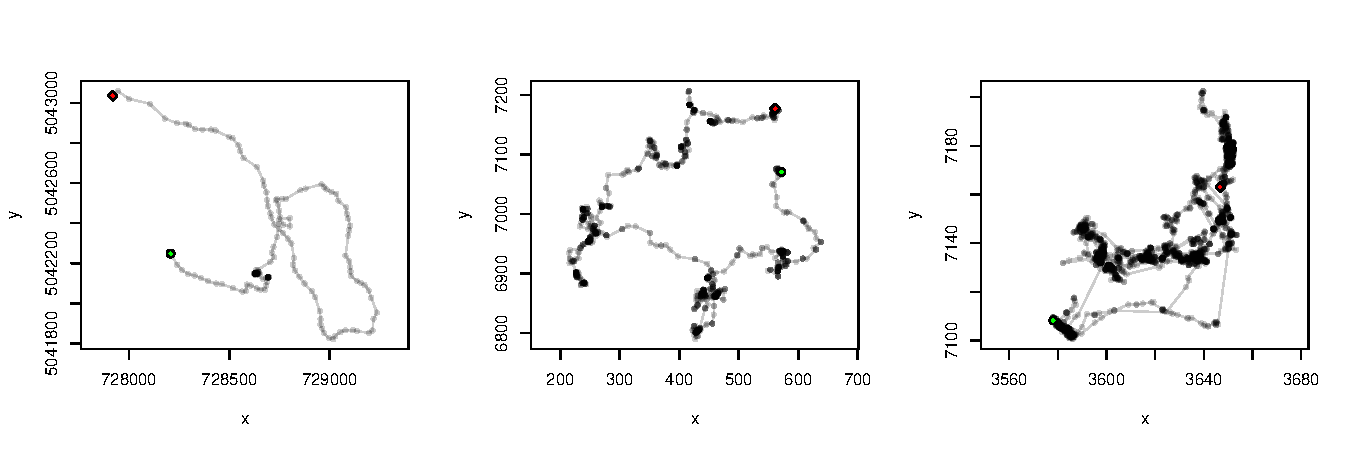
\includegraphics[width=\textwidth]{figure/alltracks} 

\end{knitrout}



\subsection{Analysis Methods}

\subsubsection{First Passage Time}

The idea of first passage time (FPT) analysis ({\bf references!}) is to straightforwardly measure the time it takes to leave a fixed radius $r$. It is used to identify intensive spatial use, especially area restricted search (ARS), but just as well denning, milling or other are restricted behaviors.  If a radius is chosen that is greater than the scale of a restricted area, the FPT is much higher when the animal is restricted than when the animal is moving.  More complex uses of FPT are to quantify a somewhat loosely defined scale of area restricted behavior by, e.g.~computing the variance of the log of FPT over a range of scales, and finding the radius where this quantity is maximized, but in our application we choose a single radius, and use the output of the FPT calculation to reduce the movement data to a simple, one-dimensional index of use intensity.  It is applied using the  `adehabitatLT' package in `R` (Calenge 2006).   

FPT analysis has only one ``tuning knob'', the parameter $r$. There are no real fundamental assumptions related to the underlying movement; however it can only detect behavioral changes that are associated with restricted use of spatial area. 


\subsubsection{Bayesian partitioning of Markovian models}

This method (which might be made into an acronym like BPMM) is an approach to segmenting of movement data that assumes that the movement (or some time-series derived from the movement data) is composed of some unknown number of pre-defined homogeneous Markovian processes (candidate models).  A Bayesian partitioning of the complete time-series into the specific series of candidate models. This approach was originally developed in molecular biology, to partition DNA sequences (Gueguen 2001) and has been adapted and implemented for movement segmentation in adehatitatLT (Calenge 2009), and is very well-documented in the accompanying ``vignette'' document, though otherwise appears to be ``underpublished''.  

Using this method entails the following steps:

\ben
\I Regularizing the data as much as possible, either interpolating or susbetting points. 
\I Choosing a movement variable to partition.  In all cases here we use the (regularized) displacement step $S$.  
\I Selecting a set of $k$ candidate models $m_1, m_2  ... m_k$.  In all cases we choose $k=20$ normal models with a range of means $\mu_j = (j/k) max(S)$, with a fixed standard deviation $\sigma = \sqrt{\text{var}{S_j}} / k$.  The method is ``Markovian'' because each of these models is a discrete behavioral state which the animal transitions between.  
\I Assessing the optimal number of partitions in the data by using a likelihood based method.  Further details are in Gueguen (2001, 2009)
\I Fitting that number of partitions (or any nubmer the used chooses) to the time-series.
\een

The ouput is a partitioning which includes the times of the changes between models, and the model selected for each partition.   The choices for the analyses here largely follow the recommendations of Calenge (unpublished) {\bf Cl\'ement: How do we cite the vignette?  The help file states that this method is ``unpublished'' ... is this still the case?}.


\subsubsection{Behavioral Changepoint Analysis}

The behavioral changepoint analysis (BCPA, Gurarie et al.~2009) uses a likelihood-based method for identifying significant changes in movement parameter values across a long and complex dataset by sweeping an analysis window over the timeseries and identifying the most likely changepoint, and which, if any, of the parameters might have changed at that changepoint.  By design, the BCPA is meant to be robust to irregularly sampled data.  

Implementing the BCPA involves the following steps (\emph{Note, there are several technical improvements over the original 2009 implementation, which might be added to an appendix}):

\ben
\I Pick a response time-series variable $X$.  One fairly robust variable is $vc = V \cos(\theta)$ where $V$ is speed = displacement/time interval and $\theta$ is turning angle.  Another alternative is simply $V$. 

\I Assume that the observations $X(t)$ are a observations from a stationary continuous-time Gaussian process with mean $\mu_i$, standard deviation $\sigma_i$ and time-scale of autocorrelation $\tau_i$, where $i \in (1,2,...N)$ represents an \emph{a priori} unknown number of behavioral states. \emph{Note: the use of a continuous time scale $\tau >0$ is a change from the original model, which estimates a discrete autocorrelation $0 < \rho < 1$.  The time-scale is more biologically meaningful, as it is estimated in units of time: the longer the time-scale the longer the ``memory'' of the movement}.

\I Obtain a likelihood for $\mu_i$, $\sigma_i$ and $\rho_i$ within a given stationary state $i$ (See Gurarie et al. 2009 for details + updates in supplementary material).

\I Find the location within a window of observations which splits a subset of the data into two sets of the three parameters. (Technical note: before I obtained all the possibilities and mixed out the maximum, not I use R's `optimize()` to find it - which is faster).

\I Within this window, use a version of BIC to determine which combination (if any) of the three parameters most parsimoniously describes the separation in the data.  Often, the null model is returned.  I say "modified" because the BIC is usually defined as: $BIC = - 2 \log(L) + k \log(n)$, where $L$ is the likelihood, $k$ is the number of parameters, and $n$ is the number of datapoint; however, the 2 I replace with a constant $K > 0$.  The smaller this value, the more conservative the analysis, i.e.~the more likely it is to select a simpler or null model.  This is one of several ``tuning knobs'' in the BCPA. 

\I Sweep a window of fixed size across the time series and collect all the changepoints, the  associated models, and the values of the estimated parameters according to the selected model on either side of the changepoint within the window.   Note, the window size is another "knob" - larger windows are more robust but more coarse, smaller windows are more sensitive but more likely to give slightly spurious results, compensated by adjusting the $K$.
\een

These steps summarize the actual analysis.  A (slight) innovation is that the output of the analysis can be summarized and presented in two ways: 
 
\ben
\I Smooth BCPA: A ``smooth'' output is the one described in the original paper: is the average over all the estimated parameters, and the location of all the change points on the other.  This gives interesting output - with, in particular, the opportunity to have parameters change both suddenly and gradually, and to visualize a phase plot of the behavioral shifts - both sudden and gradual. 

\I Flat BCPA: A "flat" output takes the result of the window sweep and finds the most frequently chosen change points, clustering those unique changepoints which are close to each other (within some interval $dT_c$).  The three parameters $\mu$, $\sigma$ and $\tau$ are then estimated within each section, and the location of these ``flat'' changepoints is recorded.  This output is directly comparable to the BPMM segmentation. 
\een

\section{Results}

I walk through the implementation of these methods systematically for the lamprey data, and present the results of the analyses applied to the wolf and wild forest reindeer.  

\subsection{Lamprey analysis: Step-by-step implementation}

The lamprey data set is the only dataset which I first smoothed, very slightly, by averaging locations over three steps. The effect of the smoothing is made more clear below:

\begin{knitrout}
\definecolor{shadecolor}{rgb}{0.969, 0.969, 0.969}\color{fgcolor}\begin{kframe}
\begin{alltt}
Smooth <- \hlfunctioncall{function}(X) \hlfunctioncall{rowMeans}(\hlfunctioncall{cbind}(X[-(1:2)], X[-\hlfunctioncall{c}(1, \hlfunctioncall{length}(X))], X[-\hlfunctioncall{c}(\hlfunctioncall{length}(X) - 
    1, \hlfunctioncall{length}(X))]))
L2 <- \hlfunctioncall{data.frame}(Time = \hlfunctioncall{as.POSIXlt}(\hlfunctioncall{Smooth}(Lamprey$Time), origin = \hlstring{"1970-01-01 00:00.00 UTC"}, 
    tz = \hlstring{"America/Detroit"}), X = \hlfunctioncall{Smooth}(Lamprey$X), Y = \hlfunctioncall{Smooth}(Lamprey$Y), Z = \hlfunctioncall{Smooth}(Lamprey$Z))
\end{alltt}
\end{kframe}
\end{knitrout}


To perform both the FPT and BPMM analyses, we use the `ltraj` data type from `adehabitatLT`:

\begin{knitrout}
\definecolor{shadecolor}{rgb}{0.969, 0.969, 0.969}\color{fgcolor}\begin{kframe}
\begin{alltt}
LampreyRaw.traj <- \hlfunctioncall{as.ltraj}(\hlfunctioncall{data.frame}(Lamprey$X, Lamprey$Y), \hlfunctioncall{as.POSIXct}(Lamprey$Time), 
    id = \hlstring{"Lamprey"})
LampreySmooth.traj <- \hlfunctioncall{as.ltraj}(\hlfunctioncall{data.frame}(L2$X, L2$Y), \hlfunctioncall{as.POSIXct}(L2$Time), 
    id = \hlstring{"Lamprey"})
\end{alltt}
\end{kframe}
\end{knitrout}


\subsubsection{FPT}

Obtaining plots of the FPT at three different radii: 5, 10 and 50 m.  

\begin{knitrout}\small
\definecolor{shadecolor}{rgb}{0.969, 0.969, 0.969}\color{fgcolor}\begin{kframe}
\begin{alltt}
r <- \hlfunctioncall{c}(5, 10, 20)
LampreyRaw.fpt <- \hlfunctioncall{fpt}(LampreyRaw.traj, r)
LampreySmooth.fpt <- \hlfunctioncall{fpt}(LampreySmooth.traj, r)

\hlfunctioncall{for} (i in 1:3) \{
    \hlfunctioncall{plot}(\hlfunctioncall{attr}(LampreyRaw.fpt[[1]], \hlstring{"date"}), LampreyRaw.fpt[[1]][, i], ylab = \hlstring{"50 km FPT"}, 
        xlab = \hlstring{""})
    \hlfunctioncall{lines}(\hlfunctioncall{attr}(LampreyRaw.fpt[[1]], \hlstring{"date"}), LampreyRaw.fpt[[1]][, i])
    \hlfunctioncall{title}(\hlfunctioncall{paste}(\hlstring{"Lamprey Raw FPT:"}, r[i], \hlstring{"m"}))
\}
\hlfunctioncall{for} (i in 1:3) \{
    \hlfunctioncall{plot}(\hlfunctioncall{attr}(LampreySmooth.fpt[[1]], \hlstring{"date"}), LampreySmooth.fpt[[1]][, i], 
        ylab = \hlstring{"50 km FPT"}, xlab = \hlstring{""})
    \hlfunctioncall{lines}(\hlfunctioncall{attr}(LampreySmooth.fpt[[1]], \hlstring{"date"}), LampreySmooth.fpt[[1]][, i])
    \hlfunctioncall{title}(\hlfunctioncall{paste}(\hlstring{"Lamprey Smooth FPT:"}, r[i], \hlstring{"m"}))
\}
\end{alltt}
\end{kframe}
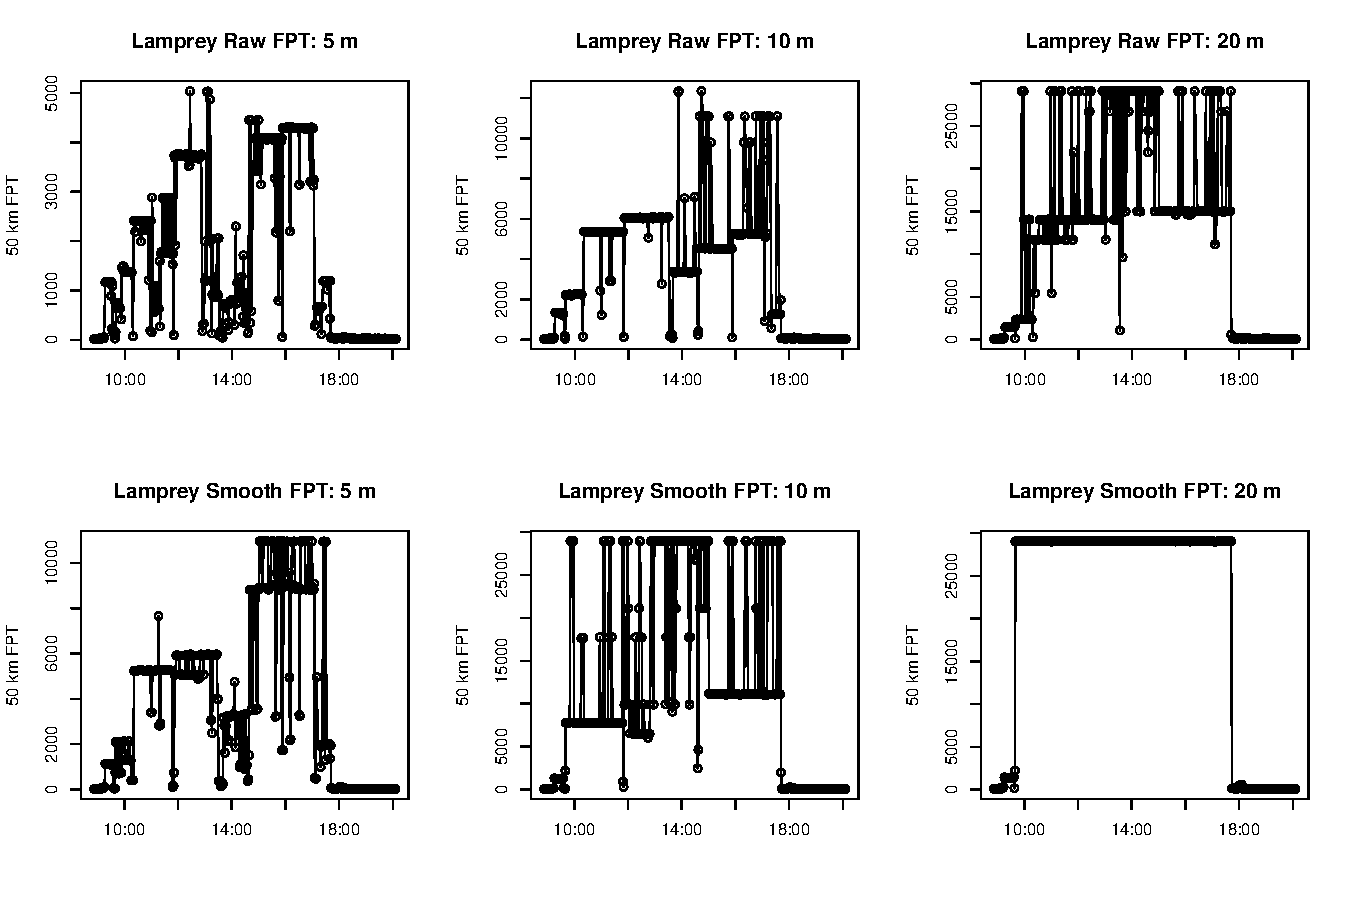
\includegraphics[width=\textwidth]{figure/FPTexample} 

\end{knitrout}


Two important conclusions from these plots: (1st) the smoothing is very important, (2nd) the 20 m radius is largely sufficient to clearly distinguish the settled period, i.e.~note the clear plateau where the first passage time is extremely high. We choose this as a suitable spatial scale for the FPT, and plot the track:  
  
\bc
\begin{knitrout}\small
\definecolor{shadecolor}{rgb}{0.969, 0.969, 0.969}\color{fgcolor}\begin{kframe}
\begin{alltt}
\hlfunctioncall{PathPlot.fpt}(LampreySmooth.traj, 20, scale = 0.1, k = 2)
\end{alltt}
\end{kframe}
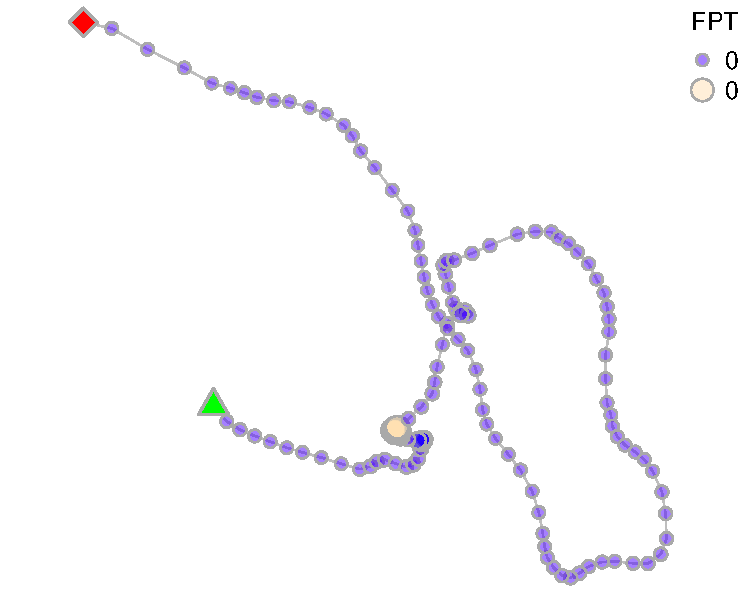
\includegraphics[width=0.6\textwidth]{figure/FPTpath} 

\end{knitrout}

\ec
The figure shows clearly the location of the spot where the lamprey settled (large pale circles with extremely high first passage time). 
  
  
  
\subsubsection{BPMM}

The following figure plots the step lengths of the lamprey movement data:

\bc
\begin{knitrout}\small
\definecolor{shadecolor}{rgb}{0.969, 0.969, 0.969}\color{fgcolor}\begin{kframe}
\begin{alltt}
\hlfunctioncall{plot}(LampreySmooth.traj[[1]]$date, LampreySmooth.traj[[1]]$dist, xlab = \hlstring{""}, 
    ylab = \hlstring{"\hlfunctioncall{Distance} (m)"}, type = \hlstring{"l"}, col = \hlstring{"darkgrey"})
\hlfunctioncall{points}(LampreySmooth.traj[[1]]$date, LampreySmooth.traj[[1]]$dist, pch = 19, 
    cex = 0.5)
\end{alltt}
\end{kframe}
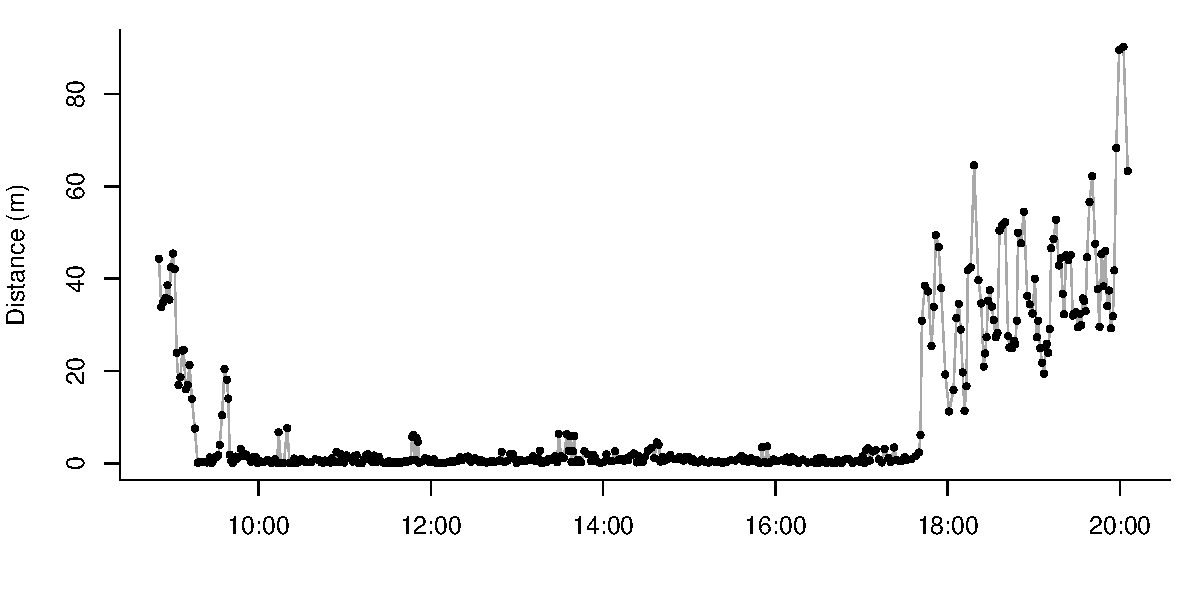
\includegraphics[width=0.7\textwidth]{figure/BPMMexample} 

\end{knitrout}

\ec

A ``visual'' inspection suggests that a standard deviation of 5 m might be appropriate for the variance within the homogeneous sections, so we use `sd = 5` (\emph{though this is clearly invalid for the stopped locations, where the sd is much lower.  Here, it does not matter so much, but for later analyses, I use the log of step length, which is much more normally distributed,  as the time series to fit.  To Do: write a diagnostic plot function to assess the model fit.}).  The `nmodels` argument sets the number of candidate models, i.e.~the $\mu_j$'s ranging from 0 to the maximum value of the step length. The first step is an assessment of the number of partitions that might be present in these data:

\bc
\begin{knitrout}\small
\definecolor{shadecolor}{rgb}{0.969, 0.969, 0.969}\color{fgcolor}\begin{kframe}
\begin{alltt}
Lamprey.reg <- \hlfunctioncall{InterpolatePoints}(Lamprey, 60)$Data
Lamprey.traj <- \hlfunctioncall{as.ltraj}(\hlfunctioncall{data.frame}(Lamprey.reg$X, Lamprey.reg$Y), Lamprey.reg$Time, 
    id = \hlstring{"Lamprey"})
Lamprey.segments <- \hlfunctioncall{PrepSegments}(Lamprey.traj, units = \hlstring{"min"}, dt = 1, sd = 5, 
    nmodels = 20)
\end{alltt}
\end{kframe}
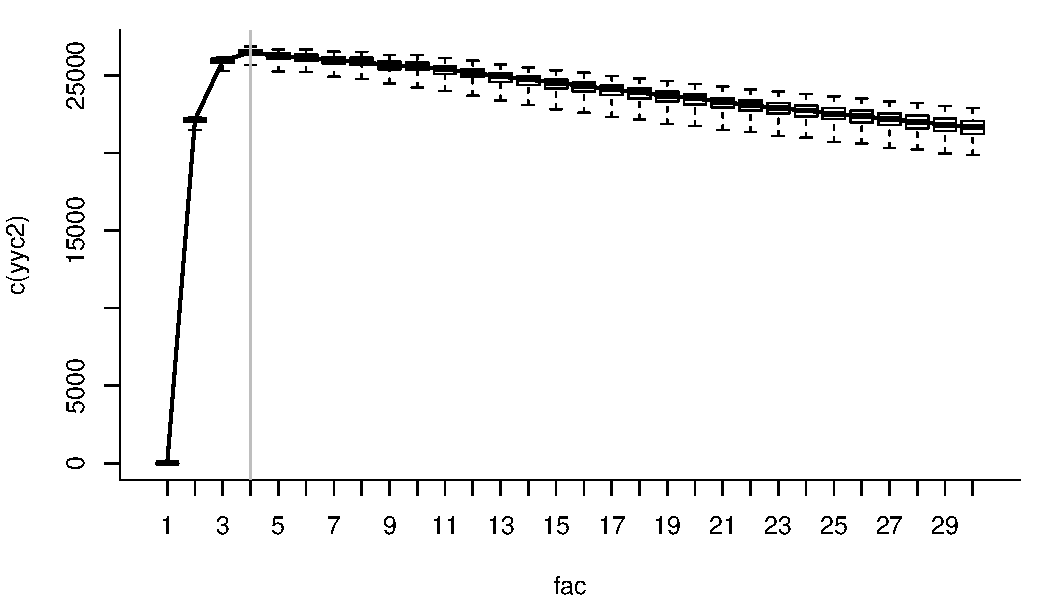
\includegraphics[width=0.7\textwidth]{figure/BPMM_likelihoods} 
\begin{kframe}\begin{verbatim}
## Maximum likelihood for K =  4
\end{verbatim}
\end{kframe}
\end{knitrout}

\ec

The likelihood assessment suggests 4 partitions - one more than the 3 partitions that we might have expected (repeated runs sometimes do suggest 3).  Note that one of the actions that occurs within  this function is a ``regularization'' of the data, i.e. coerce the time intervals to a constant 1 minute, and record missing data with NA.

We now fit the four partition model, and plot the segments.

\bc
\begin{knitrout}\small
\definecolor{shadecolor}{rgb}{0.969, 0.969, 0.969}\color{fgcolor}\begin{kframe}
\begin{alltt}
Lamprey.segments$pm <- \hlfunctioncall{PlotSegments}(Lamprey.segments, xlab = \hlstring{""}, ylab = \hlstring{"Step \hlfunctioncall{length} (m)"})
\end{alltt}
\end{kframe}
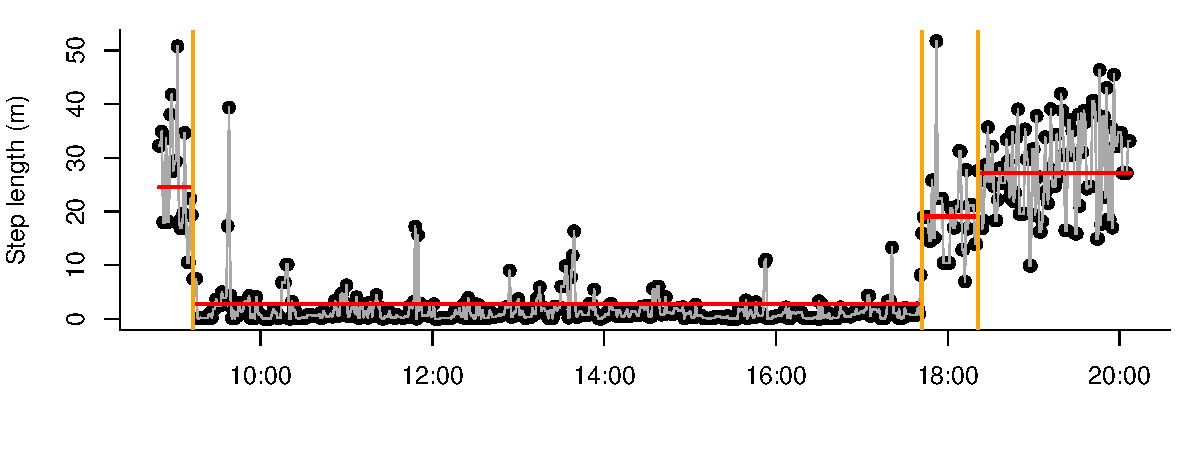
\includegraphics[width=0.7\textwidth]{figure/BPMM_segments} 

\end{knitrout}

\ec

  
Finally, the path plot according to the segmentation.  

\bc
\begin{knitrout}
\definecolor{shadecolor}{rgb}{0.969, 0.969, 0.969}\color{fgcolor}\begin{kframe}
\begin{alltt}
\hlfunctioncall{PathPlot.segments}(Lamprey.segments, where = \hlstring{"bottomleft"}, n.dots = 3, ncol = 1, 
    cex = 1.5)
\end{alltt}
\end{kframe}
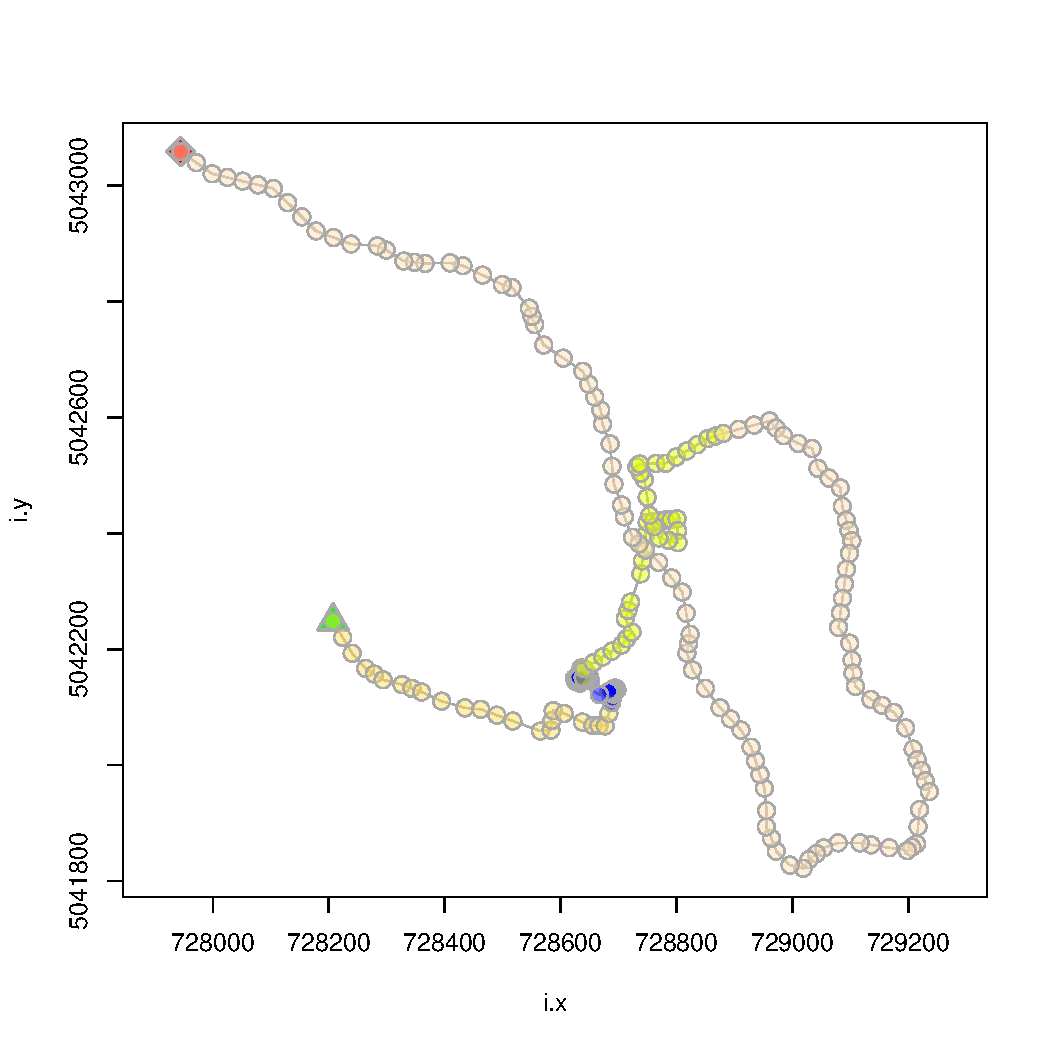
\includegraphics[width=0.5\textwidth]{figure/BPMMpath} 

\end{knitrout}

\ec

From this plot, it is clear that the fourth segment is a parsing of the movement of the lamprey as it is waking into two stages, which may be of interest to the lamprey biologists, as there is a hypothesis that they have distinct movement stages.


\subsubsection{BCPA}

To perform the BCPA, we first extract all the variables we need ($V$, turning angle $\theta$, etc.) from the Lamprey data, using the `GetVT` function:
\begin{knitrout}
\definecolor{shadecolor}{rgb}{0.969, 0.969, 0.969}\color{fgcolor}\begin{kframe}
\begin{alltt}
Lamprey.VT <- \hlfunctioncall{GetVT}(L2, units = \hlstring{"min"})
\end{alltt}
\end{kframe}
\end{knitrout}


Now we select a windowsize and sensitivity parameter K and perform the windowsweep.  Note that since the resolution of the data is mostly around one location per minute, a windowsize of 30 corresponds to a half-hour window.  

\begin{knitrout}
\definecolor{shadecolor}{rgb}{0.969, 0.969, 0.969}\color{fgcolor}\begin{kframe}
\begin{alltt}
Lamprey.ws <- \hlfunctioncall{WindowSweep}(Lamprey.VT, \hlstring{"V*\hlfunctioncall{cos}(Theta)"}, windowsize = 30, plotme = FALSE, 
    K = 0.5)
\end{alltt}
\end{kframe}
\end{knitrout}


The key portion of the output of this function is the ``windowsweep'' data frame, which contains the proposed break (last column), the parameters to the left and right of the break, and the selected model:

\begin{knitrout}
\definecolor{shadecolor}{rgb}{0.969, 0.969, 0.969}\color{fgcolor}\begin{kframe}
\begin{alltt}
\hlfunctioncall{head}(Lamprey.ws$ws)
\end{alltt}
\begin{verbatim}
##   Model     LL   bic    mu1    s1   rho1    mu2    s2   rho2 Break.bb.time
## 1     0 -86.40 53.50 11.494 12.39 20.647 11.494 12.39 20.647         27.67
## 2     0 -86.97 53.79 10.911 12.20 19.111 10.911 12.20 19.111         26.00
## 3     0 -86.35 53.48 10.608 12.06 19.074 10.608 12.06 19.074         22.17
## 4     0 -87.11 53.86 10.313 11.76 16.959 10.313 11.76 16.959         20.67
## 5     0 -85.64 53.12  9.818 11.26 16.151  9.818 11.26 16.151         19.33
## 6     0 -89.59 55.09  8.706 10.31  9.884  8.706 10.31  9.884         20.67
\end{verbatim}
\end{kframe}
\end{knitrout}


Note that in this example, the first 6 windows contained no shifts in parameter values, so the values are the same to the left and to the right of each changepoint. (A minor note: the \textt{rho1} and \textt{rho2} columns correspond to $\tau_1$ and $\tau_2$ - time-scales which are in units of minutes in this case.)  

The following functions plot the output of the ``flat'' and ``smooth'' summary respectively, 

\begin{knitrout}\small
\definecolor{shadecolor}{rgb}{0.969, 0.969, 0.969}\color{fgcolor}\begin{kframe}
\begin{alltt}
\hlfunctioncall{plot}(Lamprey.ws, type = \hlstring{"flat"}, clusterwidth = 1, legend = FALSE, xaxt = \hlstring{"n"}, 
    pt.cex = 1, ylab = \hlfunctioncall{expression}(V * \hlfunctioncall{cos}(theta)))
\hlfunctioncall{MakeLetter}(\hlstring{"Flat BCPA"}, \hlstring{"top"})
\hlfunctioncall{plot}(Lamprey.ws, type = \hlstring{"smooth"}, threshold = 5, legend = FALSE, pt.cex = 1, 
    ylab = \hlfunctioncall{expression}(V * \hlfunctioncall{cos}(theta)), col.cp = \hlfunctioncall{rgb}(0.5, 0, 0.5, 0.3))
\hlfunctioncall{MakeLetter}(\hlstring{"Smooth BCPA"}, \hlstring{"top"})
\end{alltt}
\end{kframe}
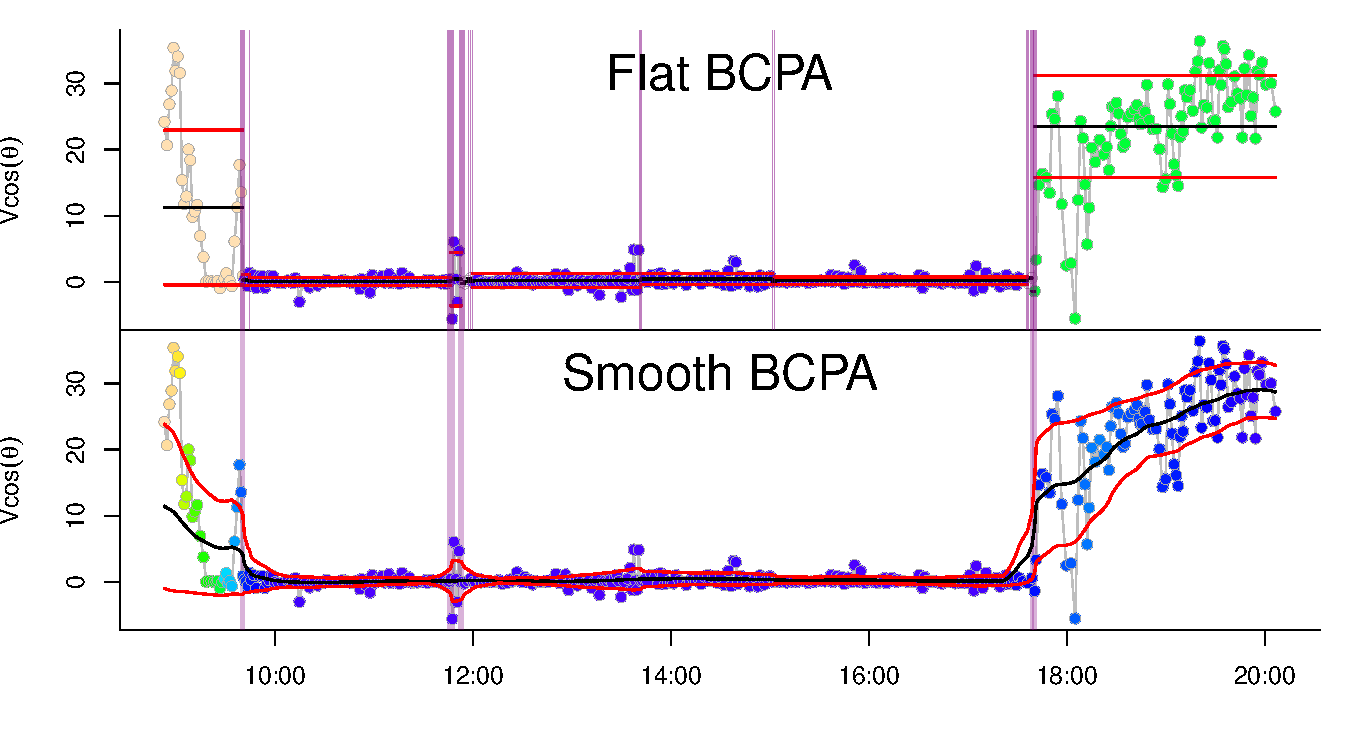
\includegraphics[width=\textwidth]{figure/BCPAsegments} 

\end{knitrout}


In these plots, the vertical lines represent the significant change points, the width of the lines is proportional to the number of time that change point was selected, the black an dred lines represent the mean and standard deviation estimate, and the colors reflect the autocorrelation time-scale (bluer colors have smaller autocorrelation time scales).

For these, relatively simple data, the BCPA clearly identifies the major transitions to settling, but also picked out a small portion of activity in the middle of the settling.  The smooth output also showed the ramping down and the ramping up of the movement.  Also, it suggests that the movements tend to be more correlated as the lamprey settles than as it ``awakes''.

The following plots are path plots of the BCPA output:
\begin{knitrout}
\definecolor{shadecolor}{rgb}{0.969, 0.969, 0.969}\color{fgcolor}\begin{kframe}
\begin{alltt}
\hlfunctioncall{PathPlot}(Lamprey, Lamprey.ws, type = \hlstring{"flat"}, clusterwidth = 4, ylab = \hlstring{""}, plotlegend = TRUE, 
    tauwhere = \hlstring{"bottomleft"}, ncol.legend = 2, axes = FALSE)
\hlfunctioncall{MakeLetter}(\hlstring{"Flat BCPA"}, \hlstring{"top"})

\hlfunctioncall{PathPlot}(Lamprey, Lamprey.ws, type = \hlstring{"smooth"}, plotlegend = TRUE, tauwhere = \hlstring{"bottomleft"}, 
    ncol.legend = 2, axes = FALSE, ylab = \hlstring{""})
\hlfunctioncall{MakeLetter}(\hlstring{"Smooth BCPA"}, \hlstring{"top"})
\end{alltt}
\end{kframe}
\end{knitrout}


The width of the line is proportional to the mean speed, while the colors correspond to the time-scales in the plots above.  You can clearly see the lower-speed, more highly correlated settling, compared to the less correlated but higher speed leaving.  \emph{Note to lamprey folk: That lower correlation may be related to the casting behavior.}

Note that for the BCPA (as for the BBFM), it is possible to assess the assumptions, i.e.~see if the standardized residuals of the final model are indeed distributed roughly as ${\cal N}(0,1)$ random variables

\begin{knitrout}
\definecolor{shadecolor}{rgb}{0.969, 0.969, 0.969}\color{fgcolor}\begin{kframe}
\begin{alltt}
\hlfunctioncall{DiagPlot}(Lamprey.ws)
\end{alltt}
\end{kframe}
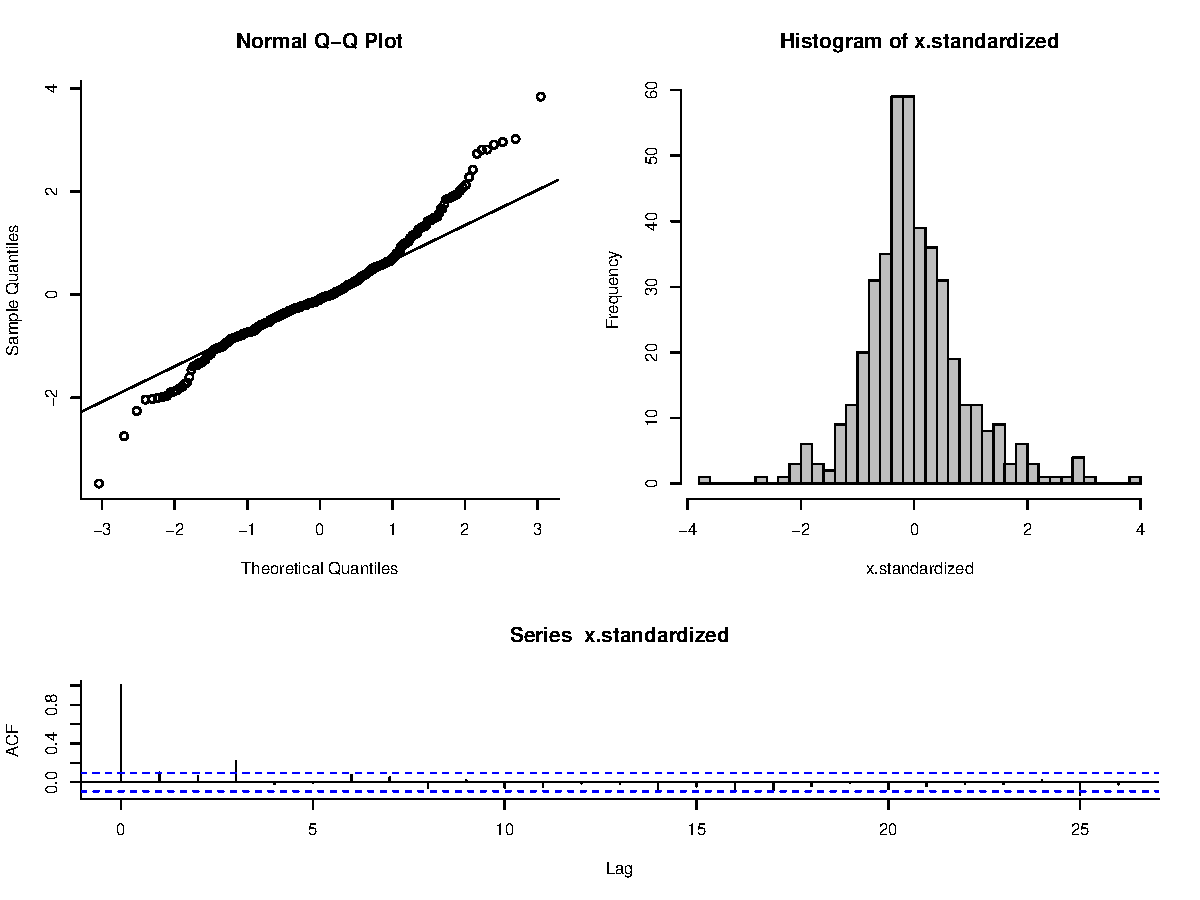
\includegraphics[width=0.8\textwidth]{figure/DiagnosticPlot} 

\end{knitrout}

\ec

This plot illustrates the qq-norm plot, the histogram and the auto-correlation function of the standardized data ($Z_i = X_i - \widehat{\mu}(T_i) / \widehat{\sigma}(T_i)$).  There is some evidence of fat tails (which can lead to spurious changepoints), but overall the results seem to satisfy the assumptions of normality. 


\subsection{Wolf and wild forest reindeer analysis}

For the wolf and reindeer analysis, I present the final time-series and path-plots for side-by-side comparison of the method, listed in the table below the parameters used for each of the analyses.  Note that for both data-sets, I additionally reduced the data (which were sampled at intervales ranging from 2 to 8 hours) to the average daily position.  Also, for the BPMM, we used the log of the step-lengths, which comforms much more closely to the normal assumption. 


\begin{tabular}{l|lll}
  Model & Setting & {\bf Wolf} ($n = 317$) & {\bf Wild forest Reindeer} ($n = 799$)\\ 
\hline \hline
\bf FPT & $r$ & 50 km  & 50 km \\
&&&  \\
\hline
\bf BPMM & $\sigma$     & 0.125  & 0.25 \\
     & N.models         & 10     & 10 \\
     & N.partitions     & 35$^*$ & 39$^*$\\
\hline
\bf BCPA & window size    & 20     & 20 \\
         & sensitivity (K)& 1      & 1 \\
         & cluster width  & 3 days & 3 days\\
\end{tabular}

The asterix in the table (next to N.partitions) refers to a setting that was automatically computed by an algorithm.  The results of these analyses are presented in the plots on the following pages.  There are long, complex paths, with a lot of structure.  However, many consistencies and patterns do appear.  For example, in the reindeer there is a strong seasonal cycle of activity during early winter (December) and late spring; however, the signature is somewhat unique between years. The wolf has several periods of virtually no activity (in late May, a week in July, most of August, a week in November).  These periods correspond to very specific and distant regions of intensive use (high first passage time).  

\subsubsection{Wolf results}
\bc
\begin{knitrout}
\definecolor{shadecolor}{rgb}{0.969, 0.969, 0.969}\color{fgcolor}
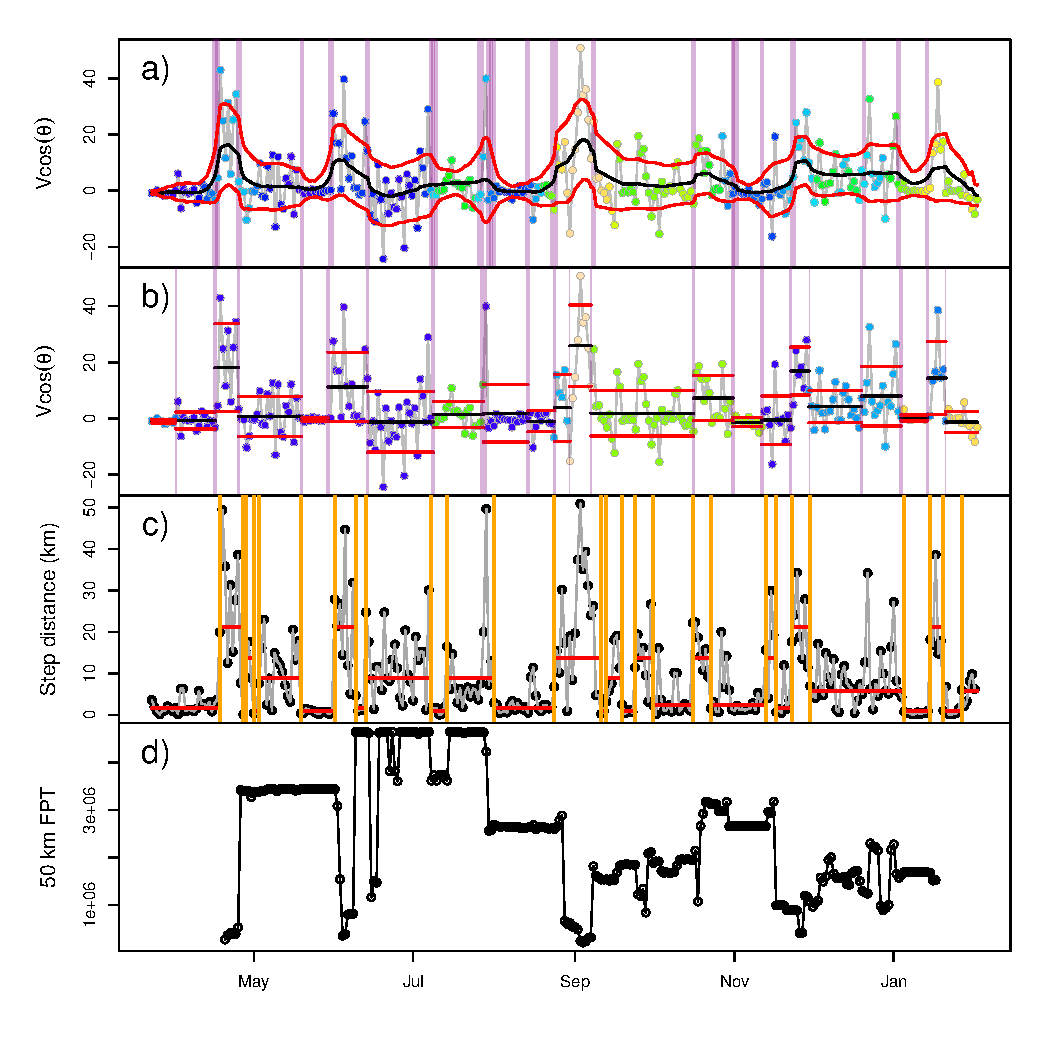
\includegraphics[width=.7\textwidth]{figure/WolfResults1} 

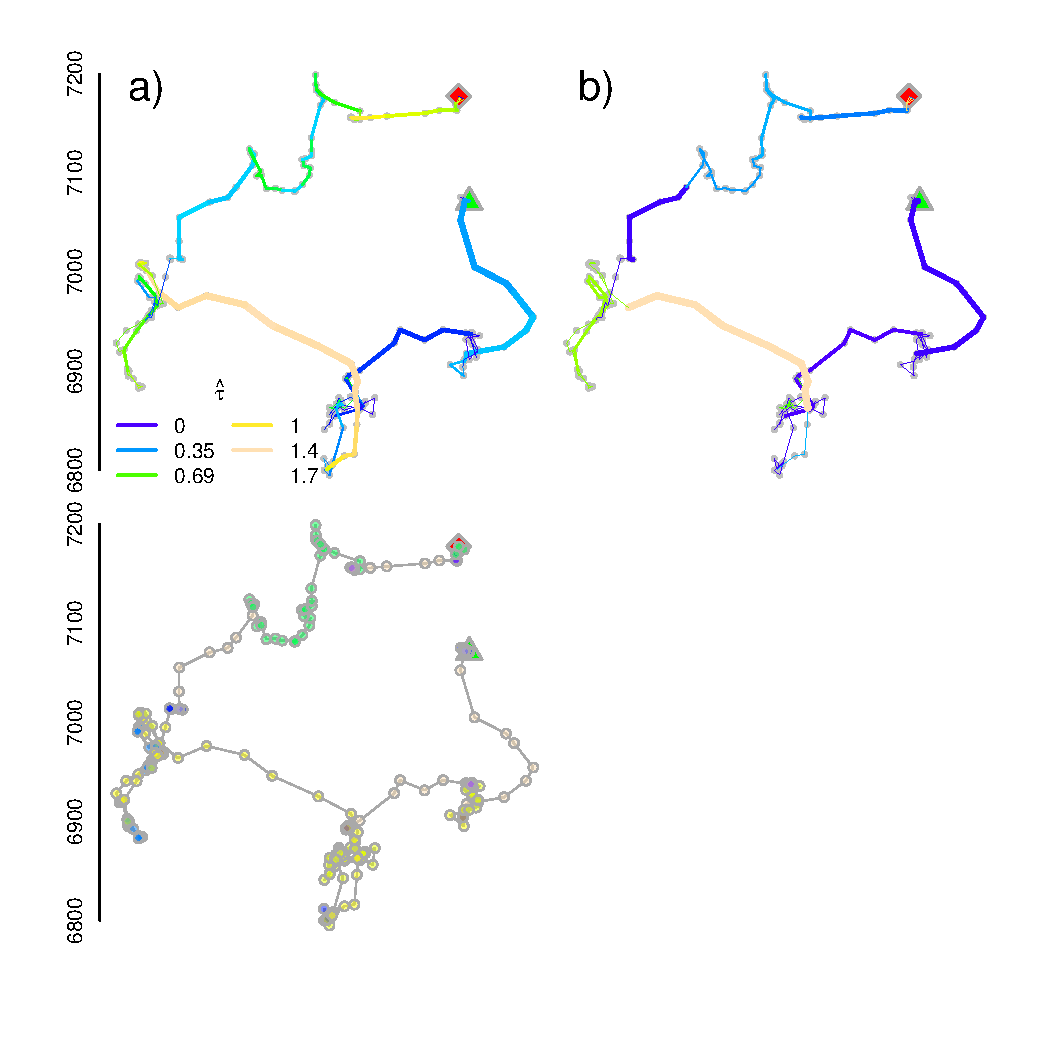
\includegraphics[width=.7\textwidth]{figure/WolfResults2} 

\end{knitrout}

\ec
\clearpage
\subsubsection{Wild forest reindeer results}
\bc
\begin{knitrout}
\definecolor{shadecolor}{rgb}{0.969, 0.969, 0.969}\color{fgcolor}
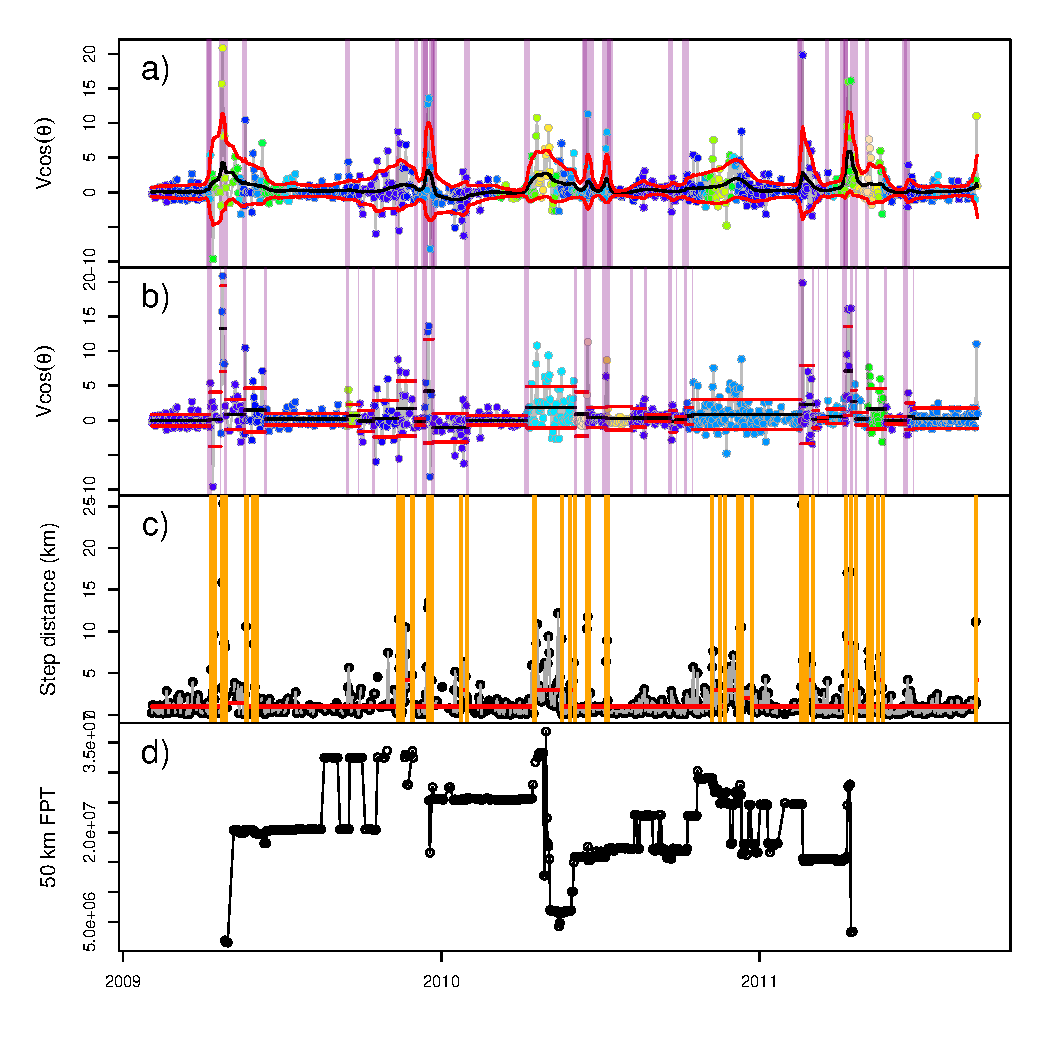
\includegraphics[width=.7\textwidth]{figure/WFRResults1} 

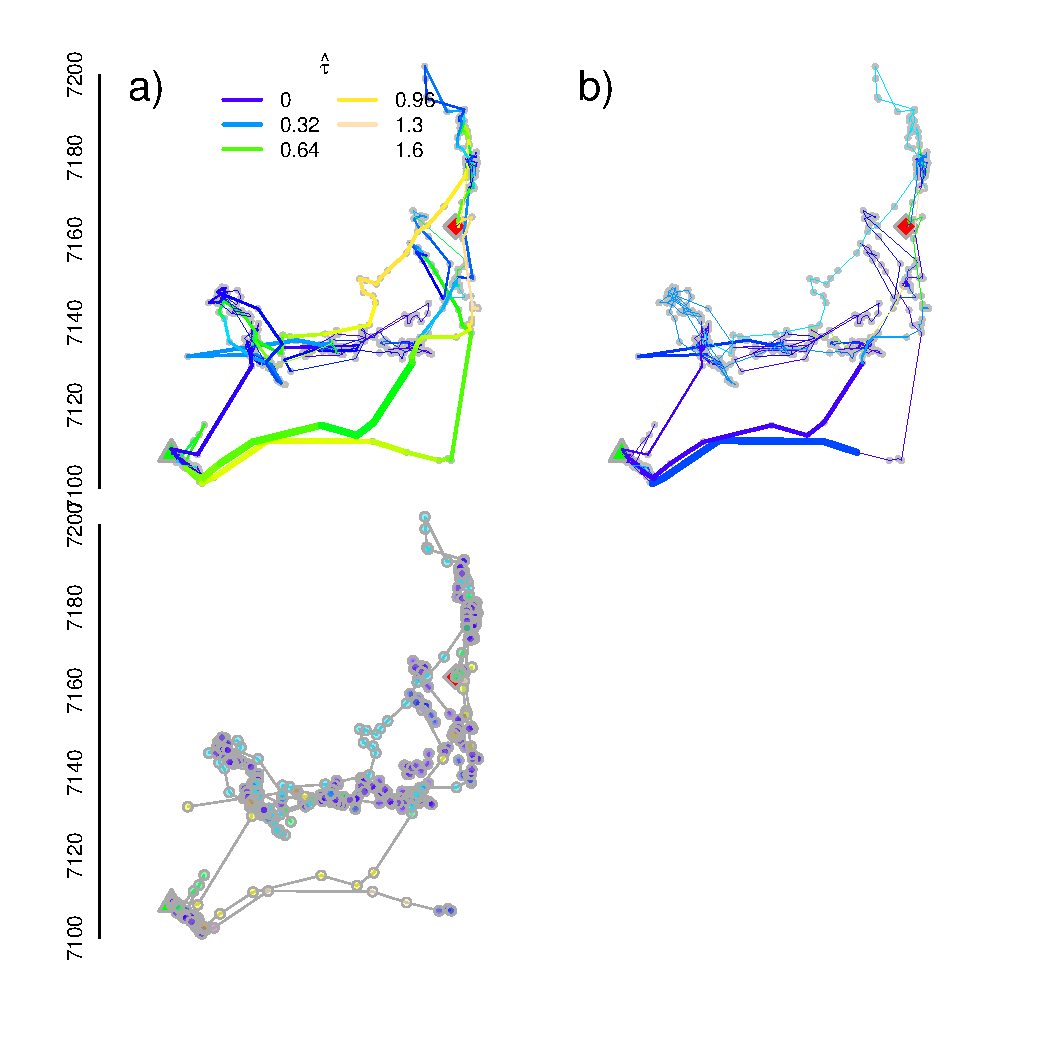
\includegraphics[width=.7\textwidth]{figure/WFRResults2} 

\end{knitrout}

\ec
\section{Discussion}

Here is a shortlist of criteria by which I'd like to compare the methods:

\ben
  \I Intensity of preprocessing
  \I Strength of assumptions
  \I Ease of implementation
  \I Ease of interpretation
  \I How mechanistic is it
\een

THe methods here, along with a hopefully-to-be included Hidden Markov Model (HMM), each are excellent in some aspects, and weak in others.  


Several conclusions / discussion points come to mind: 
\ben 
  \I The appropriate method depends in an important way on the question being asked.  For example, very specific and simple questions (e.g.~is the lamprey swimming?) the simplest tool (FPT) is by far the most effective.  Questions related to space use are somewhat different than questions related to movement metrics. 
  \I Movement behavior in general can be quite complex!  One immediate utility of all of these tools (but especially BPMM and BCPA) is to visually explore the patterns of movement.  As an exploratory tool it can serve to motivate more complex, process-based models. 
  \I The more complex the process, the stronger the assumptions that you have to make!
  \I These methods can all be improved in several ways.  In particular, the BPMM and BCPA could both quite readily fit a mechanistic movement model (like the HMM - though the model there is very simplistic), as long as a likelihood is well defined.
\een

\large \emph{That's as far as I've gotten!  Any and all additional ideas are EXTREMELY welcome!}

\normalsize

\section{References}
\begin{description}

\item Calenge, C. 2006. The package adehabitat for the R software: a tool for the analysis of space and habitat use by animals. Ecological Modelling, 197, 516-519
\item Calenge, C., Gueguen, L., Royer, M. and Dray, S. (unpublished) Partitioning the trajectory of an animal with Markov models.
\item Fauchald, P. and Tveraa, T. 2003. Using first-passage time in the analysis of area-restricted search and habitat selection.  Ecology, 84, 282-288.
\item Gueguen, L. 2001. Segmentation by maximal predictive partitioning according to composition biases. Pp 32-44 in: Gascuel, O. and Sagot, M.F. (Eds.), Computational Biology, LNCS, 2066.
\item Gueguen, L. 2009. Computing the likelihood of sequence segmentation under Markov modelling. Arxiv preprint arXiv:0911.3070.
\item Gurarie, E., R. Andrews and K. Laidre. 2009. A novel method for identifying behavioural changes in animal movement data. Ecol. Lett. 12: 395-408.

\end{description}


\end{document}


\end{document}
